\setlength\parindent{0pt} % no indentation for the entire note

\subsection{state function}
A function that describes the \emph{equilibrium} state of a system (e.g., energy, internal energy,
enthalpy, entropy, pressure, temperature, volume, chemical composition, density, etc) irrespective
of how the system arrived in the state. e.g, $f(p,V,T)=0$. Whereas, mechnical work and heat depends
on the \emph{path} between two equilibrium states. \\

\subsection{process function}
{\bf{Derivation}}: Values that depends on the path (e.g., time) of two equilibrium states (e.g.,
work, and heat).

\subsection{ideal gas}
For $n$ moles of any gas
\begin{equation}
    pV = nR^*T,
\end{equation}
with the universal constant $R^*$ [$J K^{-1}$ mol$^{-1}$]. We know that $n=1$ mole of dry air equals
$M_d$ (molecular weight for dry air) grams of dry air, $1[\text{mol}] = M_d [0.001\text{kg}]$,
\begin{equation}
        p_d V_d  = M_d \Big(\frac{1000 R^*}{M_d} [ J K^{-1} \text{kg}^{-1}]\Big) T \\
\end{equation}
which becomes
\begin{equation} \label{eq:idealgas2}
    p_d \alpha_d = R_d T.
\end{equation}
This is the general relationship of any gas, hence the water vapor pressure 
\begin{equation} \label{eq:idealgas3}
   e \alpha_v = R_v T.
\end{equation}


\subsection{internal energy}
{\bf{Definition}}: $I(S,V,\{N_i\})$, composed of kinetic and potential energy of the molecules and
atoms. The change depends only on the initial and final states of the system. Can not be directly
measured, but can be prepared by taking partial derivative of entropy, volume, and its mole number.

\subsection{internal energy (dry ideal gas)}
{\bf{Definition}}: d$I = c_v$ d$T$, the internal energy soley depends on temperature, not
volume/density/pressure. \\

{Joule's experiment:} \\
In a free expansion ($p_iV_i = p_fV_f$, pressure change is completely balanced by volume change),
d$W = 0$, d$Q = 0$ hence d$I = 0$, and from the ideal gas equation the temperature stays constant
(since the molecules rarely meet even before the expansion, so the kinetic energy, which is affected
solely by temperature for ideal gas, remains constant). We can therefore conclude that internal
energy is solely governed by temperature. We can imagine this conclusion by using two Joule's
experiment by using the same volume compartment begining with two different temperatures, which
gives two internal energies in the end of expansion. 


\subsection{heat}
{\bf{Definition}}: Heat is energy ``transferred" between two objects or systems in thermal contact, not
a state to a single system. Do not confuse heating rate as a time derivative of a function of state.


\subsection{heat (dry ideal gas)}
{\bf{Derivation}}: From first law of thermodynamics for a unit mass of dry ideal gas
\begin{equation} \label{eq:energy_cv}
\begin{aligned}
  \td Q & = \td I + \td W \\
        & = c_v \td T + p \td \alpha \\
        & = c_v \td T + \td(p\alpha) - \alpha \td p \\
        & = \td (c_v T + p\alpha) - \alpha \td p. 
\end{aligned}
\end{equation}
The first term is heat change due to change in {\bf{enthalpy}}, $h = I + p\alpha$, at constant
pressure. Where change in internal energy/temperature and volume take effect. The second
term is heat change at constant temperature due to pressure change. Further derivation 
\begin{equation} \label{eq:energy_cp}
\begin{aligned}
  \td Q & = (c_v + R) \td T - \alpha \td p
        & = c_p \td T - \alpha \td p
\end{aligned}
\end{equation}
shows that the heat capacity under constant pressure and constant volume could be associated by
\begin{equation}
  \big( \frac{\td q}{\td T} \big)_p = \frac{\td h}{\td T} =  c_p = c_v + R.
\end{equation}

\subsection{thermodynamic equation}
For general {\clr non-ideal gas}, by combining continuity equation and
\begin{equation}
    \frac{DI}{Dt} + p \frac{D\alpha}{Dt} = \dot{Q}, 
\end{equation}
results in the internal energy equation
\begin{equation}
    \boxed{\frac{DI}{Dt} + p\alpha \nabla \cdot v = \dot{Q}}.
\end{equation}
and the pressure term (also missing the dynamics in the momentum equation) could be obtained
diagnostically as
\begin{equation}
   p = -\frac{\partial I}{\partial \alpha},
\end{equation}
where $\alpha$ dynamics is from continuity equation. \\

As for {\clr ideal gas}, 
\begin{equation}
    c_v\frac{DT}{Dt} + p \frac{D\alpha}{Dt} = \dot{Q}, \ \text{or} \ \ 
    c_p\frac{DT}{Dt} + \alpha \frac{Dp}{Dt} = \dot{Q},
\end{equation}
one would obtain a thermodynamic equation for $T$ and solve for $p$ by $p = \rho R T$. Which is
by combining the continuity equation with
\begin{equation}
    \frac{DI}{Dt} - \frac{RT}{\rho} \frac{D\rho}{Dt} = \dot{Q},
\end{equation}
and result in the temperature equation
\begin{equation}
    \boxed{c_v\frac{DT}{Dt} + RT \nabla \cdot v = \dot{Q}}.
\end{equation}
If further large scale \emph{\clr hydrostatic balance} $\alpha \td p = -g \td z$ is assumed, then the
thermodynamic equation pertains to the dry static energy $\td Q = \td (c_v T + gz) = \td s$, 
\begin{equation}
   \boxed{\frac{Ds}{Dt} = \dot{Q}}.
\end{equation}

\subsection{potential temperature (dry ideal gas)}
{\bf{Definition}}: $\theta = \frac{p_0}{p}^\kappa$, this is obtained by setting $\td Q=0$ and
integrate \eqref{eq:energy_cp}. 

\subsection{equivalent potential temperature}
{\bf{Definition}}: $\theta_e$, the temperature obtained by condensing out all the vapor. \\

{\bf{Derivation}}: From first law, 
\begin{equation}
\begin{aligned}
   \td Q & = c_p \td T - \alpha \td p \\ 
         & = c_p \td T - RT \td \ln p \\
         & = c_p( \td T - \frac{RT}{c_p} \td \ln p) \\
         & = c_p( \td T + T \td \ln(\frac{p_0}{p})^\kappa 
\end{aligned}
\end{equation}
when substituting $\td Q = -L\td q_{vs}$ and divide by $c_p T$ this becomes, 
\begin{equation}
\begin{aligned}
   \frac{-L}{c_pT} \td q_{vs} & = \td \ln T + \td \ln(\frac{p_0}{p})^\kappa \\
          & = \ln (T(\frac{p_0}{p})^\kappa) = \td \ln \theta.
\end{aligned}
\end{equation}
Integrate from saturation to all moisture condensed out ($q_{vs}=0$) results in the equivalent potential
temperature
\begin{equation}
\begin{aligned}
   \boxed{\theta_e = \theta(T,p) \exp(\int_0^{q_{vs}} \frac{L}{c_pT} \td q_{vs})}.
\end{aligned}
\end{equation}

\subsection{reversible process}
In thermodynamics term, a process ``taken place" is defined as transition from intial to final
state. A reversible process is if this process can be reversed without additional work, and causes
no change to the system or surrounding environment. 

\subsection{entropy}
A measure of ``difference'' between adiabats (no heat exchange processes), and a measure of ``work
loss'' in transferring heat (irreversible process). \\

In a closed system, when heat is added at a constant temperature (volume expands and pressure
decreases), the amount of disorder increases which increases the potential temperature (the actual
temperature is higher when forced back to original pressure). For a irreversible process, suppose a
heat reservoir at $T_2$ transfers heat $Q$ to a cooler reservoir at $T_0$. By Carnot's engine, we
know that the maximum available energy the heat tranferred into work is
\begin{equation}
    W_2 = (1-\frac{T_0}{T_2})Q.
\end{equation}

For a irreversible process (state variables (e.g., p, V, T) cannot go back to original values
without additional work), where heat is first transferred to a middle reservoir at the state $T_1 <
T_2$, and then transfers the same amount of heat $Q$ to the cold reservoir at $T_0$.
Notice since $T_1 < T_2$, therefore the entropy is higher to transfer the same amount of $Q$.
Therefore the maximum available work from the middle reservoir is
\begin{equation}
    W_1 = (1-\frac{T_0}{T_1})Q,
\end{equation}
which is less than $W_2$. Hence, the work loss from irreversible process is 
\begin{equation}
    W_2-W_1 = Q(T_0/T_1 - T_0/T_2) = T_0(S_1 - S_2) = T_0 dS,
\end{equation} 
in a form of heat loss, where the increase in $dS$ becomes a measure of work loss. 
%A sum of entropy gain of $S_1$ from the middle reservoir and 
%entropy loss of $S_2$ from the original reservoir in the irreversible process.
There is a net gain in entropy in the irreversible process.
i.e., {\bf the more entropy gain/more disorderness contributes to more work loss, which becomes a
less efficient process.}

\subsection{specific volume}
{\bf Definition}: $v = 1/\rho$, volume occupied by 1kg of mass.

\subsection{mixing ratio}
{\bf Definition}: $ \frac{m_i}{m_{\text{tot}}-m_i} $.

\subsection{water vapor mixing ratio}
{\bf Definition}: $ q = \frac{m_v}{m_d}$, actual mass mixing ratio between vapor and dry air.

\subsection{saturation mixing ratio}
{\bf Definition}: $ q_s = \frac{m_{vs}}{m_d}$, maximum amount of water vapor allowed in the dry air.

\subsection{latent heat}
{\bf Definition}: $Q$ [kJ], energy released/absorbed by a body during a constant temperature process
(phase transition).

\subsection{specific latent heat}
{\bf Definition}: $L$ [kJ/kg]= $Q/m$, amount of heat required to complete phase change of a unit
mass of substance.

\subsection{Clausius-Claperon Relation}
{\bf Definition}: $\frac{\Delta P}{\Delta T} = \frac{L}{T\Delta v}$, P-T coexistence curve slope
relation. Under typical atmoshperic conditions, 
\begin{equation}
   \frac{d e_s}{dT} = \frac{L_v(T)e_s}{R_vT^2}, 
\end{equation}
where: $L_v$ is latent heat for evaporation varying with $T$, $R_v$ is the water vapor gas constant.
\\


\subsection{saturation vapor pressure}
August-Roche-Magnus formula (approximation from Clausius-Claperon Relation): \\
\begin{equation}
   e_s(T) = 6.1094 \text{exp}(\frac{17.625T}{T+243.04}).
\end{equation}
( water-holding capacity of the atmosphere increases by about $7\%$ for every $1^{\circ}$C heated )

\subsection{unsaturated vapor pressure}
{\bf Definition}: $e = \frac{(n_{\text{air}} + n_{\text{water}})}{V}RT$, 

\subsection{relative humidity}
{\bf Definition}: $RH = \frac{e}{e_s}(T)$.

\subsection{virtual temperature}

{\bf Definition}: $T_v(p,\rho)$, temperature at which a dry parcel would have at $p$ and $\rho$ of a
moist parcel. \\

{\bf Derivation}: Suppose a moist parcel has density $\rho$ and pressure $p$.
Dalton's law of partial pressure gives $p = e + p_d$, combined with \eqref{eq:idealgas2} and
\eqref{eq:idealgas3} give
\begin{equation}
   \rho = \frac{m_d + m_v}{V} = \rho_d + \rho_v = \frac{p-e}{R_dT} + \frac{e}{R_vT}, 
\end{equation}
where $\rho_d$ and $\rho_v$ are the partial densities.
Solving this gives
\begin{equation}
   {\clr p} = {\clr \rho} R_d \frac{T}{1-\frac{e}{p}(1-\frac{R_d}{R_v})} = \rho R_d {\clr T_v},
\end{equation}
where, $\frac{R_d}{R_v} \approx 0.622$ in the atmosphere. \\

{\bf Purpose}:
The gas constant for moist air (a mix of pure water vapor and dry air) depends strongly on the
amount of water vapor, so it is convenient to use a fictitious temperature with the dry-air equation
of state to represent how "heavy" a moist parcel is (i.e., the more water vapor means a dry air
needs to heat more to reach same pressure and density to become "light"). \\

\subsection{lifting condensation level (LCL)}
{\bf Definition}: $z_l$, height at which an unsaturated parcel reaches saturation, $RH=100\%$, dry
adiabatically, then starts following moist adiabatic lapse rate upward. 
\begin{figure} [H] 
   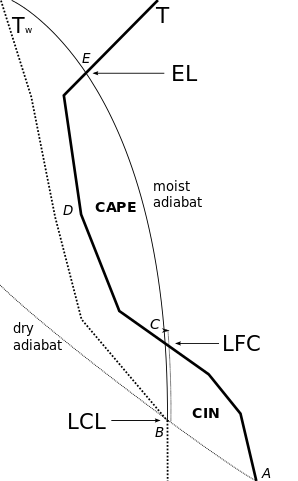
\includegraphics[width=0.2\textwidth, height=0.3\textwidth]{sounding.png}
   \caption{\label{sounding}}
\end{figure}

\subsection{level of free convection (LFC)}
{\bf Definition}: $z_f$, height at which a moist parcel temperature is equal to the environment,
and temperature increases faster than the environment. \\

{\bf Example}: The unsaturated parcel in Figure {\ref{sounding}} is lifted dry adiabatically from A
to B to saturation, and further lifted moist adiabatically to C until surpassing the environmental
temperature.

\subsection{equilibrium level (EL)}
{\bf Definition}: $z_e$, height at which the moist parcel lapse rate is greater than environment.

\subsection{dew point/condensate temperature}
{\bf Definition}: $T_d$, temperature at LCL when a parcel reaches $RH=100\%$ by expansion cooling.

\subsection{wet bulb temperature}
{\bf Definition}: $T_w$, the temperature when saturation is reached in a bulb of moist ambient air
and a wet cloth through evaporative cooling, i.e., air cooled by cloth warming (measure taken from
the air). \\ 

{\bf Interpretation}: $T_w$ is reached by evaporative cooling, whereas $T_d$ is
reached by expansion cooling (constant pressure). $T_d \le T_w$ since when a parcel saturates by
evaporation, the dew point inside increases which is higher than the original dew point $T_d$.

\subsection{convective inhibition (CIN)}
{\bf Definition}: 
CIN $=\int_{z_0}^{z_f} g \frac{T_{v,\text{parcel}} - T_{v,\text{env}}}{T_{v,\text{env}}} $d$z$, 
a negative energy value measuring how much a parcel is prevented to rise to LFC from the surface. \\

{\bf Interpretation}: The term $\frac{T_{v,\text{parcel}}}{T_{v,\text{env}}} -
1$ shows when the parcel is moister (larger $T_{v,\text{parcel}}$, more buoyant), CIN is less negative.

\subsection{convective available potential energy (CAPE)}
{\bf Definition}: 
CAPE $=\int_{z_f}^{z_e} g \frac{T_{v,\text{parcel}} - T_{v,\text{env}}}{T_{v,\text{env}}} $d$z$,
differs from CIN in just the levels of integration.




